\documentclass{beamer}
\usepackage[utf8]{inputenc}
\usepackage{graphicx, epsfig}
\usepackage{amsmath,mathrsfs,amsfonts,amssymb}
%\usepackage{subfig}
\usepackage{floatflt}
\usepackage{epic,ecltree}
\usepackage{mathtext}
\usepackage{fancybox}
\usepackage{fancyhdr}
\usepackage{multirow}
\usepackage{enumerate}
\usepackage{epstopdf}
\usepackage{multicol}
\usepackage{algorithm}
\usepackage[noend]{algorithmic}
\def\algorithmicrequire{\textbf{Input:}}
\def\algorithmicensure{\textbf{Output:}}
\usetheme{default}%{Singapore}%{Warsaw}%{Warsaw}%{Darmstadt}
\usecolortheme{default}
\setbeamertemplate{footline}[page number]{}
\setbeamerfont{title}{size=\Huge}

\newcommand{\bt}{\mathbf{t}} 
\newcommand{\bu}{\mathbf{u}} 
\newcommand{\bw}{\mathbf{w}} 
\newcommand{\bx}{\mathbf{x}} 
\newcommand{\bz}{\mathbf{z}} 
\newcommand{\by}{\mathbf{y}} 

\newcommand{\bI}{\mathbf{I}} 
\newcommand{\bT}{\mathbf{T}} 
\newcommand{\bX}{\mathbf{X}} 
\newcommand{\bZ}{\mathbf{Z}} 

\newcommand{\bepsilon}{\boldsymbol{\epsilon}} 
\newcommand{\bmu}{\boldsymbol{\mu}} 
\newcommand{\bphi}{\boldsymbol{\phi}} 
\newcommand{\bSigma}{\boldsymbol{\Sigma}} 
\newcommand{\btheta}{\boldsymbol{\theta}} 

\DeclareMathOperator*{\argmin}{arg\,min}
\DeclareMathOperator*{\argmax}{arg\,max}

%\definecolor{beamer@blendedblue}{RGB}{15,120,80}
%----------------------------------------------------------------------------------------------------------
\title[\hbox to 56mm{Deep Generative Models  \hfill\insertframenumber\,/\,\inserttotalframenumber}]
{Deep Generative Models \\ Lecture 3}
\author[Roman Isachenko]{\\Roman Isachenko}
\institute[MIPT]{Moscow Institute of Physics and Technology \\
}
\date{2020}
%--------------------------------------------------------------------------------
\begin{document}
%--------------------------------------------------------------------------------
\begin{frame}
%\thispagestyle{empty}
\titlepage
\end{frame}
%--------------------------------------------------------------------------------
\section{Intro}
%=======
\begin{frame}{Generative models zoo}
    \begin{figure}
        \centering
        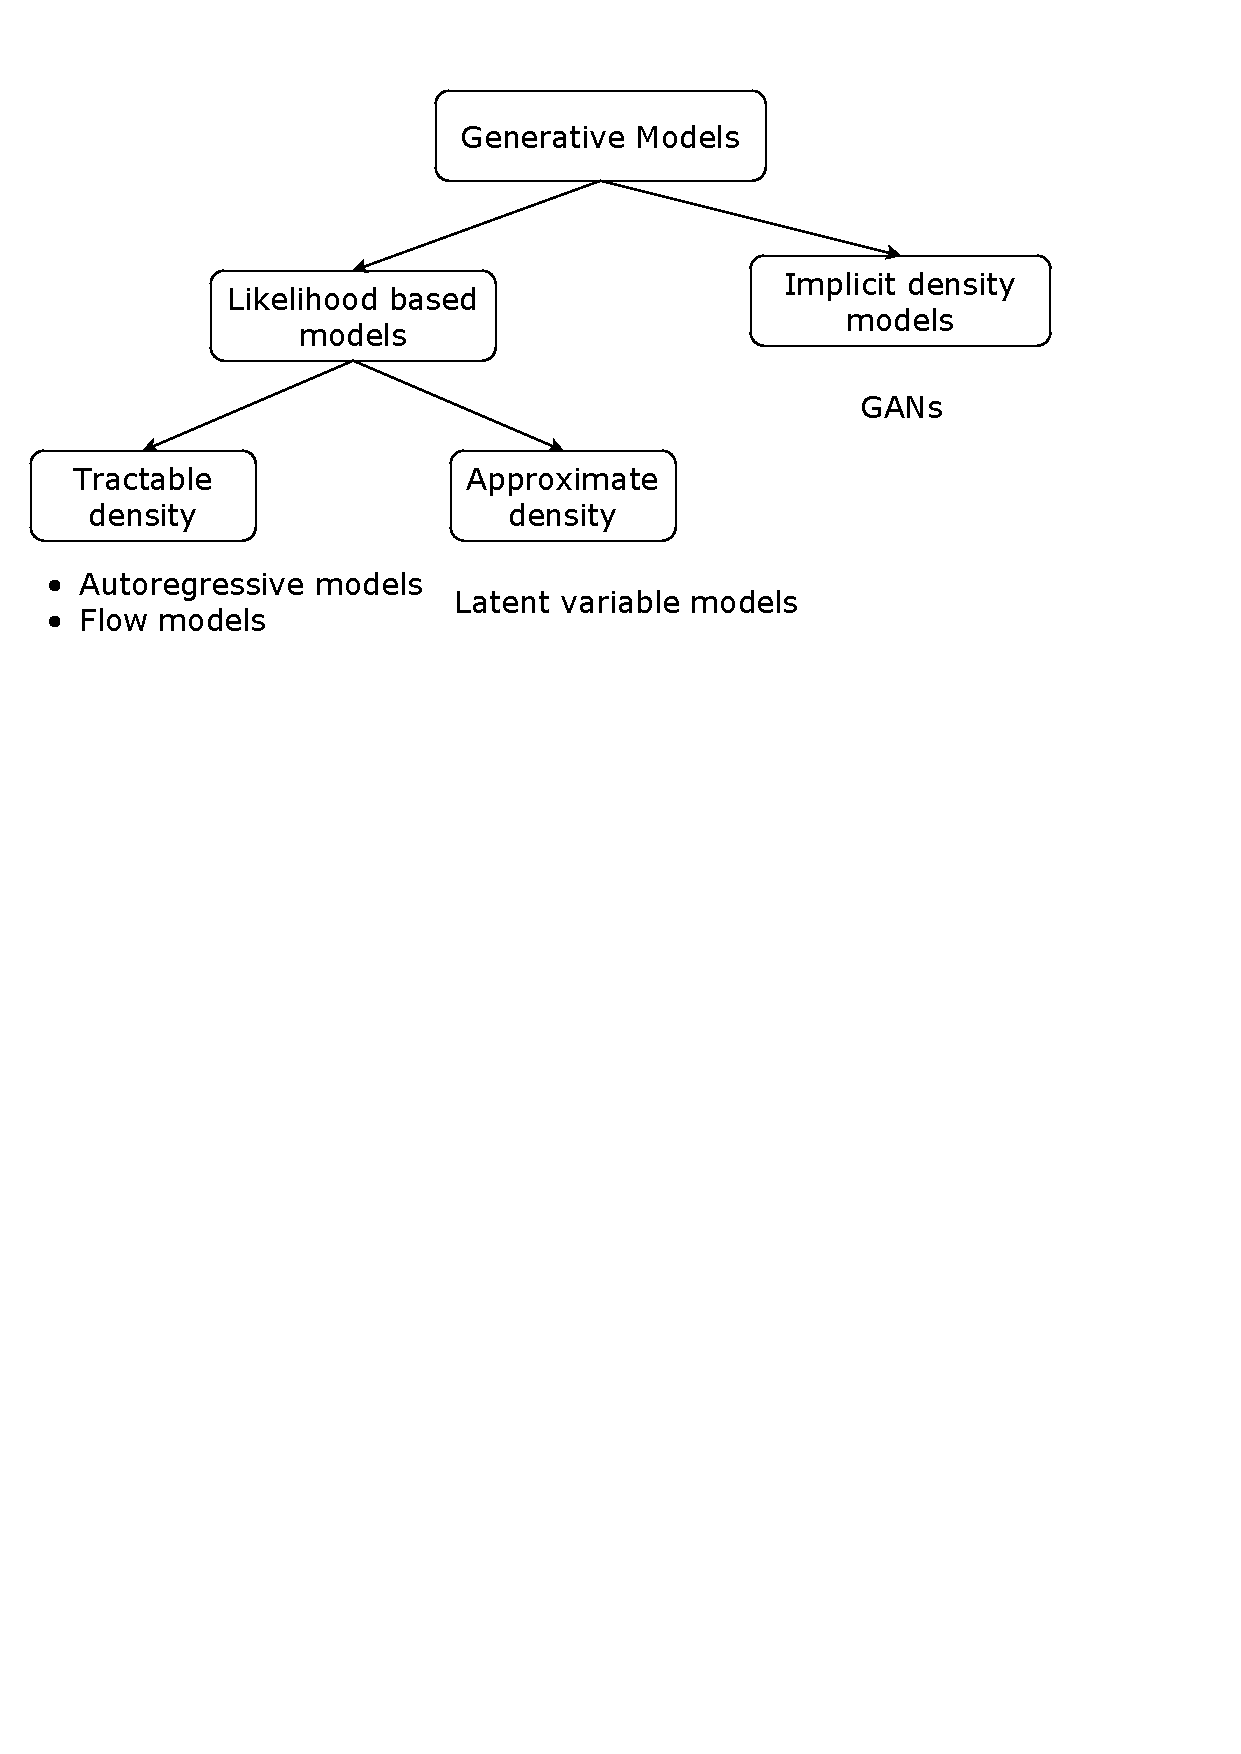
\includegraphics[width=1.0\linewidth]{figs/generative_models_zoo.pdf}
        \label{fig:generative_models_zoo}
    \end{figure}
\vfill
\hrule\medskip
{\scriptsize Radford A., Metz L., Chintala S. Unsupervised representation learning with deep convolutional generative adversarial networks  \href{https://arxiv.org/abs/1511.06434}{https://arxiv.org/abs/1511.06434}}
\end{frame}
%=======
\begin{frame}{Latent variable models}
	\begin{block}{MLE problem}
		\vspace{-0.3cm}
		\[
		\btheta^* = \argmax_{\btheta} p(\bX | \btheta) = \argmax_{\btheta} \prod_{i=1}^n p(\bx_i | \btheta) = \argmax_{\btheta} \sum_{i=1}^n \log p(\bx_i | \btheta).
		\]
		\vspace{-0.3cm}
	\end{block}
	\begin{block}{Challenge}
		$p(\bx | \btheta)$ could be intractable.
	\end{block}
	\begin{block}{Extend probabilistic model}
		Introduce latent variable $\bz$ for each sample $\bx$
		\[
		p(\bx, \bz | \btheta) = p(\bx | \bz, \btheta) p(\bz); \quad 
		\log p(\bx, \bz | \btheta) = \log p(\bx | \bz, \btheta) + \log p(\bz).
		\]
		\[
		p(\bx | \btheta) = \int p(\bx, \bz | \btheta) d\bz = \int p(\bx | \bz, \btheta) p(\bz) d\bz.
		\]
	\end{block}
\end{frame}
%=======
\begin{frame}{Incomplete likelihood}
\begin{block}{MLE problem}
	\vspace{-0.3cm}
	\begin{multline*}
		\vspace{-0.3cm}
		\btheta^* = \argmax_{\btheta} p(\bX, \bZ | \btheta) = \argmax_{\btheta} \prod_{i=1}^n p(\bx_i, \bz_i | \btheta) = \\ = \argmax_{\btheta} \sum_{i=1}^n \log p(\bx_i, \bz_i | \btheta).
	\end{multline*}
	\vspace{-0.3cm}
\end{block}
Since $\bZ$ is unknown, maximize \textbf{incomplete likelihood}.
\begin{block}{MILE problem}
	\vspace{-0.3cm}
	\begin{multline*}
		\btheta^* = \argmax_{\btheta} \log p(\bX| \btheta) = \argmax_{\btheta} \log \int p(\bX, \bZ | \btheta) d \bZ = \\ = \argmax_{\btheta} \log \int p(\bX| \bZ, \btheta) p(\bZ) d\bZ.
	\end{multline*}
	\vspace{-0.3cm}
\end{block}

\end{frame}
%=======
\subsubsection{Variational inference}
\begin{frame}{Variational lower bound}
\begin{multline*}
	\log p(\bX| \btheta) 
	= \log \frac{p(\bX, \bZ| \btheta)}{p(\bZ|\bX, \btheta)} = \\ 
	= \int q(\bZ) \log \frac{p(\bX, \bZ| \btheta)}{p(\bZ|\bX, \btheta)}d\bZ
	= \int q(\bZ) \log \frac{p(\bX, \bZ| \btheta) q(\bZ)}{p(\bZ|\bX, \btheta) q(\bZ)} d\bZ = \\
	= \int q(\bZ) \log \frac{p(\bX, \bZ | \btheta)}{q(\bZ)}d\bZ + \int q(\bZ) \log \frac{q(\bZ)}{p(\bZ|\bX, \btheta)}d\bZ = \\ 
	= \mathcal{L} (q, \btheta) + KL(q(\bZ) || p(\bZ|\bX, \btheta)) \geq \mathcal{L} (q, \btheta).
\end{multline*}
\begin{block}{Kullback-Leibler divergence}
	\begin{itemize}
		\item $KL(q || p) \geq 0$;
		\item $KL(q || p) = 0 \Leftrightarrow q \equiv p$.
	\end{itemize}
\end{block}
\end{frame}
%=======
\begin{frame}{Variational lower bound}
	\begin{block}{ELBO}
		\vspace{-0.1cm}
		\[
		\log p(\bX| \btheta) = \mathcal{L} (q, \btheta) + KL(q(\bZ) || p(\bZ|\bX, \btheta)) \geq \mathcal{L} (q, \btheta).
		\]
	\end{block}
	Instead of maximizing incomplete likelihood, maximize ELBO
	\[
		\max_{\theta} p(\bX | \btheta) \quad \rightarrow \quad \max_{q, \theta} \mathcal{L} (q, \btheta).
	\]
	\vspace{-0.4cm}
	\begin{block}{EM-algorithm}
		\begin{itemize}
			\item Initialize $\btheta^*$;
			\item E-step
			\[
			q(\bZ) = \argmax_q \mathcal{L} (q, \btheta^*) = \argmin_q KL(q || p) =
			p(\bZ| \bX, \btheta^*);
			\]
			\item M-step
			\[
			\btheta^* = \argmax_{\btheta} \mathcal{L} (q, \btheta);
			\]
			\item Repeat E-step and M-step until convergence.
		\end{itemize}
	\end{block}

\end{frame}
%=======
\begin{frame}{Amortized variational inference}
	\begin{block}{E-step}
		\vspace{-0.3cm}
		\[
		q(\bZ) = \argmax_q \mathcal{L} (q, \btheta^*) = \argmin_q KL(q || p) =
		p(\bZ| \bX, \btheta^*).
		\]
		could be \textbf{intractable}.
	\end{block}
	\begin{block}{Idea}
		Restrict the family of all possible distributions $q(\bz)$ to the particular parametric class conditioned of sample: $q(\bz|\bx, \bphi)$.
	\end{block}
	
	\textbf{Variational EM-algorithm}
	\begin{itemize}
		\item E-step
		\[
		\bphi_k = \bphi_{k-1} + \left.\eta \nabla_{\bphi} \mathcal{L}(\bphi, \btheta_{k-1})\right|_{\bphi=\bphi_{k-1}}
		\]
		\item M-step
		\[
		\btheta_k = \btheta_{k-1} + \left.\eta \nabla_{\btheta} \mathcal{L}(\bphi_k, \btheta)\right|_{\btheta=\btheta_{k-1}}
		\]
	\end{itemize}
\end{frame}
%=======
\begin{frame}{Variational EM-algorithm}

	\begin{block}{ELBO}
		\vspace{-0.1cm}
		\[
		\log p(\bX| \btheta) = \mathcal{L} (q, \btheta) + KL(q(\bZ) || p(\bZ|\bX, \btheta)) \geq \mathcal{L} (q, \btheta).
		\]
	\end{block}
	\begin{itemize}
		\item E-step
		\[
		\bphi_k = \bphi_{k-1} + \left.\eta \nabla_{\bphi} \mathcal{L}(\bphi, \btheta_{k-1})\right|_{\bphi=\bphi_{k-1}},
		\]
		where $\bphi$~-- parameters of variational distribution $q(\bz | \bx, \bphi)$.
		\item M-step
		\[
		\btheta_k = \btheta_{k-1} + \left.\eta \nabla_{\btheta} \mathcal{L}(\bphi_k, \btheta)\right|_{\btheta=\btheta_{k-1}},
		\]
		where $\btheta$~-- parameters of likelihood $p(\bx | \bz, \btheta)$.
	\end{itemize}
	Now all we have to do is to obtain two gradients $\nabla_{\bphi} \mathcal{L}(\bphi, \btheta)$, $\nabla_{\btheta} \mathcal{L}(\bphi, \btheta)$.  \\
	\textbf{Difficulty:} number of samples $n$.
\end{frame}
%=======
\begin{frame}{ELBO gradient (M-step, $\nabla_{\btheta} \mathcal{L}(\bphi, \btheta)$)}
\vspace{-0.3cm}
\[
	\mathcal{L} (\bphi, \btheta)  = \mathbb{E}_{q} \log p(\bX | \bZ, \btheta) - KL (q(\bZ| \bX, \phi) || p(\bZ)) \rightarrow \max_{\bphi, \btheta}.
\]
Optimization w.r.t. $\btheta$: \textbf{mini-batching} (1) + \textbf{Monte-Carlo} estimation (2)
\begin{align*}
	\nabla_{\btheta} \mathcal{L} (\bphi, \btheta)
	&= \sum_{i=1}^n \int q(\bz_i|\bx_i, \bphi) \nabla_{\btheta}\log p(\bx_i|\bz_i, \btheta)  d \bz_i \\
	&\mathrel{\stackrel{\rm (1)}\approx} n\int q(\bz_i|\bx_i, \bphi) \nabla_{\btheta}\log p(\bx_i|\bz_i, \btheta) d \bz_i , \quad i \sim U[1, n] \\
	&\mathrel{\stackrel{\rm (2)}\approx}  n \nabla_{\btheta}\log p(\bx_i|\bz^*_i, \btheta), \quad \bz^*_i \sim q(\bz_i|\bx_i, \bphi).
\end{align*}
\textbf{Monte-Carlo} estimation (2):
\[
	\int q(\bz) f(\bz) d\bz \approx f(\bz^*), \text{where } \bz^* \sim q(\bz).
\]
\end{frame}
%=======
\begin{frame}{ELBO gradient (E-step, $\nabla_{\bphi} \mathcal{L}(\bphi, \btheta)$)}
\vspace{-0.3cm}
\[
	\mathcal{L} (\bphi, \btheta)  = \mathbb{E}_{q} \log p(\bX | \bZ, \btheta) - KL (q(\bZ| \bX, \phi) || p(\bZ)) \rightarrow \max_{\bphi, \btheta}.
\]
	Difference from M-step: density function $q(\bz| \bx, \bphi)$ depends on the parameters $\bphi$, it is impossible to use Monte-Carlo estimation:
	\[
		\nabla_{\bphi} \mathcal{L} (\bphi, \btheta) = \int \nabla_{\bphi} q(\bZ| \bX, \bphi) \log p(\bX |\bZ, \btheta) d\bZ - \nabla_{\bphi} KL
	\]
	
	\begin{block}{Log-derivative trick}
	    \[
	    \nabla_\xi q(\eta| \xi) = q(\eta | \xi) \left( \frac{\nabla_\xi q(\eta | \xi)}{q(\eta| \xi)} \right) = q(\eta | \xi) \nabla_\xi \log q(\eta| \xi).
	    \]
	\end{block}
	\[
		\nabla_{\bphi} q(\bZ| \bX, \bphi) = q(\bZ| \bX, \bphi) \nabla_{\bphi} \log q(\bZ| \bX, \bphi).
	\]
\end{frame}
%=======
\begin{frame}{ELBO gradient (E-step, $\nabla_{\bphi} \mathcal{L}(\bphi, \btheta)$)}

	\begin{multline*}
		\nabla_{\bphi} \mathcal{L} (\bphi, \btheta) = \int \nabla_{\bphi} q(\bZ| \bX, \bphi) \log p(\bX |\bZ, \btheta) d\bZ  - \nabla_{\bphi} KL = \\ 
		=  \int q(\bZ| \bX, \bphi) \bigl[  \nabla_{\bphi} \log q(\bZ| \bX, \bphi) \log p(\bX |\bZ, \btheta) \bigr] d\bZ - \nabla_{\bphi} KL
	\end{multline*}
	After applying log-reparametrization trick, we are able to use Monte-Carlo estimation:
	\[
		\nabla_{\bphi} \mathcal{L} (\bphi, \btheta) \approx n \nabla_{\bphi} \log q(\bz_i^*| \bx_i, \bphi) \log p(\bx_i |\bz_i^*, \btheta) - \nabla_{\bphi} KL,
	\]
	\[
		\bz_i^* \sim q(\bz_i| \bx_i, \bphi).
	\]
	\vspace{-0.2cm}
	\begin{block}{Problem} 
	Unstable solution with huge variance.
	\end{block}
	\begin{block}{Solution}
	    Reparametrization trick
	\end{block}
\end{frame}
%=======
\begin{frame}{ELBO gradient (E-step, $\nabla_{\bphi} \mathcal{L}(\bphi, \btheta)$)}
\begin{block}{Reparametrization trick}
\vspace{-0.3cm}
\[
	f(\xi) = \int q(\eta|\xi) h(\eta) d\eta
\]
Let $\eta = h(g(\xi, \epsilon))$, where $g$ is a deterministic function, $\epsilon$ is a random variable with a density function $r(\epsilon)$.
\begin{multline*}
\nabla_\xi \int q(\eta|\xi) h(\eta) d\eta = \nabla_\xi \int r(\epsilon) h(g(\xi, \epsilon)) d \epsilon \\
\approx \nabla_\xi h(g(\xi, \epsilon^*)), \quad \epsilon^* \sim r(\epsilon).
\end{multline*}
\end{block}
\vspace{-0.1cm}
\begin{block}{Example}
\vspace{-0.3cm}
\[
	q(\eta|\xi) = \mathcal{N}(\eta| \mu, \sigma^2), \quad r(\epsilon) = \mathcal{N}(\epsilon|0, 1), \quad \eta = \sigma \cdot \epsilon + \mu, \quad \xi = [\mu, \sigma].
\]
\end{block}
\end{frame}
%=======
\begin{frame}{ELBO gradient (E-step, $\nabla_{\bphi} \mathcal{L}(\bphi, \btheta)$)}
	\vspace{-0.3cm}
	\begin{multline*}
		\nabla_{\bphi} \mathcal{L} (\bphi, \btheta) = \nabla_{\bphi}\int q(\bZ|\bX, \bphi) \log p(\bX| \bZ, \btheta)d\bZ  - \nabla_{\bphi} KL \\ \approx  n \nabla_{\bphi}\int r(\epsilon) \log p(\bx_i| g(\bx_i, \epsilon, \bphi), \btheta)d\epsilon  - \nabla_{\bphi} KL  \\ \approx
		n \nabla_{\bphi} \log p(\bx_i| g(\bx_i, \bepsilon^*, \bphi), \btheta)  - \nabla_{\bphi} KL , \quad \bepsilon^* \sim r(\bepsilon).
	\end{multline*}
	
	\begin{block}{Variational assumption}
	\[
	q(\bz| \bx, \bphi) = \mathcal{N} (\bmu(\bx), \boldsymbol{\Sigma}(\bx)).
	\]
	\[
		\bz = g(\bx, \bepsilon, \bphi) = \sqrt{\bSigma(\bx)} \cdot \bepsilon + \bmu(\bx).
	\]
	\end{block}
	$\nabla_{\bphi} KL (q(\bZ | \bX, \bphi) || p(\bZ))$ has an analytical solution.
\end{frame}
%=======
\begin{frame}{Variational autoencoder (VAE)}
	\begin{block}{Final algorithm}
		\begin{itemize}
			\item pick $i \sim U[1, n]$;
			\item compute stochastic gradient w.r.t. $\bphi$
				\begin{multline*}
					\nabla_{\bphi} \mathcal{L} (\bphi, \btheta) = n \nabla_{\bphi} \log p(\bx_i | g(\bx_i, \bepsilon^*, \bphi), \btheta) - \\ - \nabla_{\bphi} KL (q(\bz_i|\bx_i, \bphi) || p(\bz_i)), \quad \bepsilon^* \sim r(\bepsilon);
				\end{multline*}
			\item compute stochastic gradient w.r.t. $\btheta$
			\[
			\nabla_{\btheta} \mathcal{L} (\bphi, \btheta) = n \nabla_{\btheta} \log p(\bx_i|\bz^*_i, \btheta), \quad \bz^*_i \sim q(\bz_i|\bx_i, \bphi);
			\]
			\item update $\btheta, \bphi$ according to the selected optimization method (SGD, Adam, RMSProp).
		\end{itemize}
	\end{block}
\end{frame}
%=======
\begin{frame}{Variational autoencoder (VAE)}

\begin{figure}[h]
	\centering
	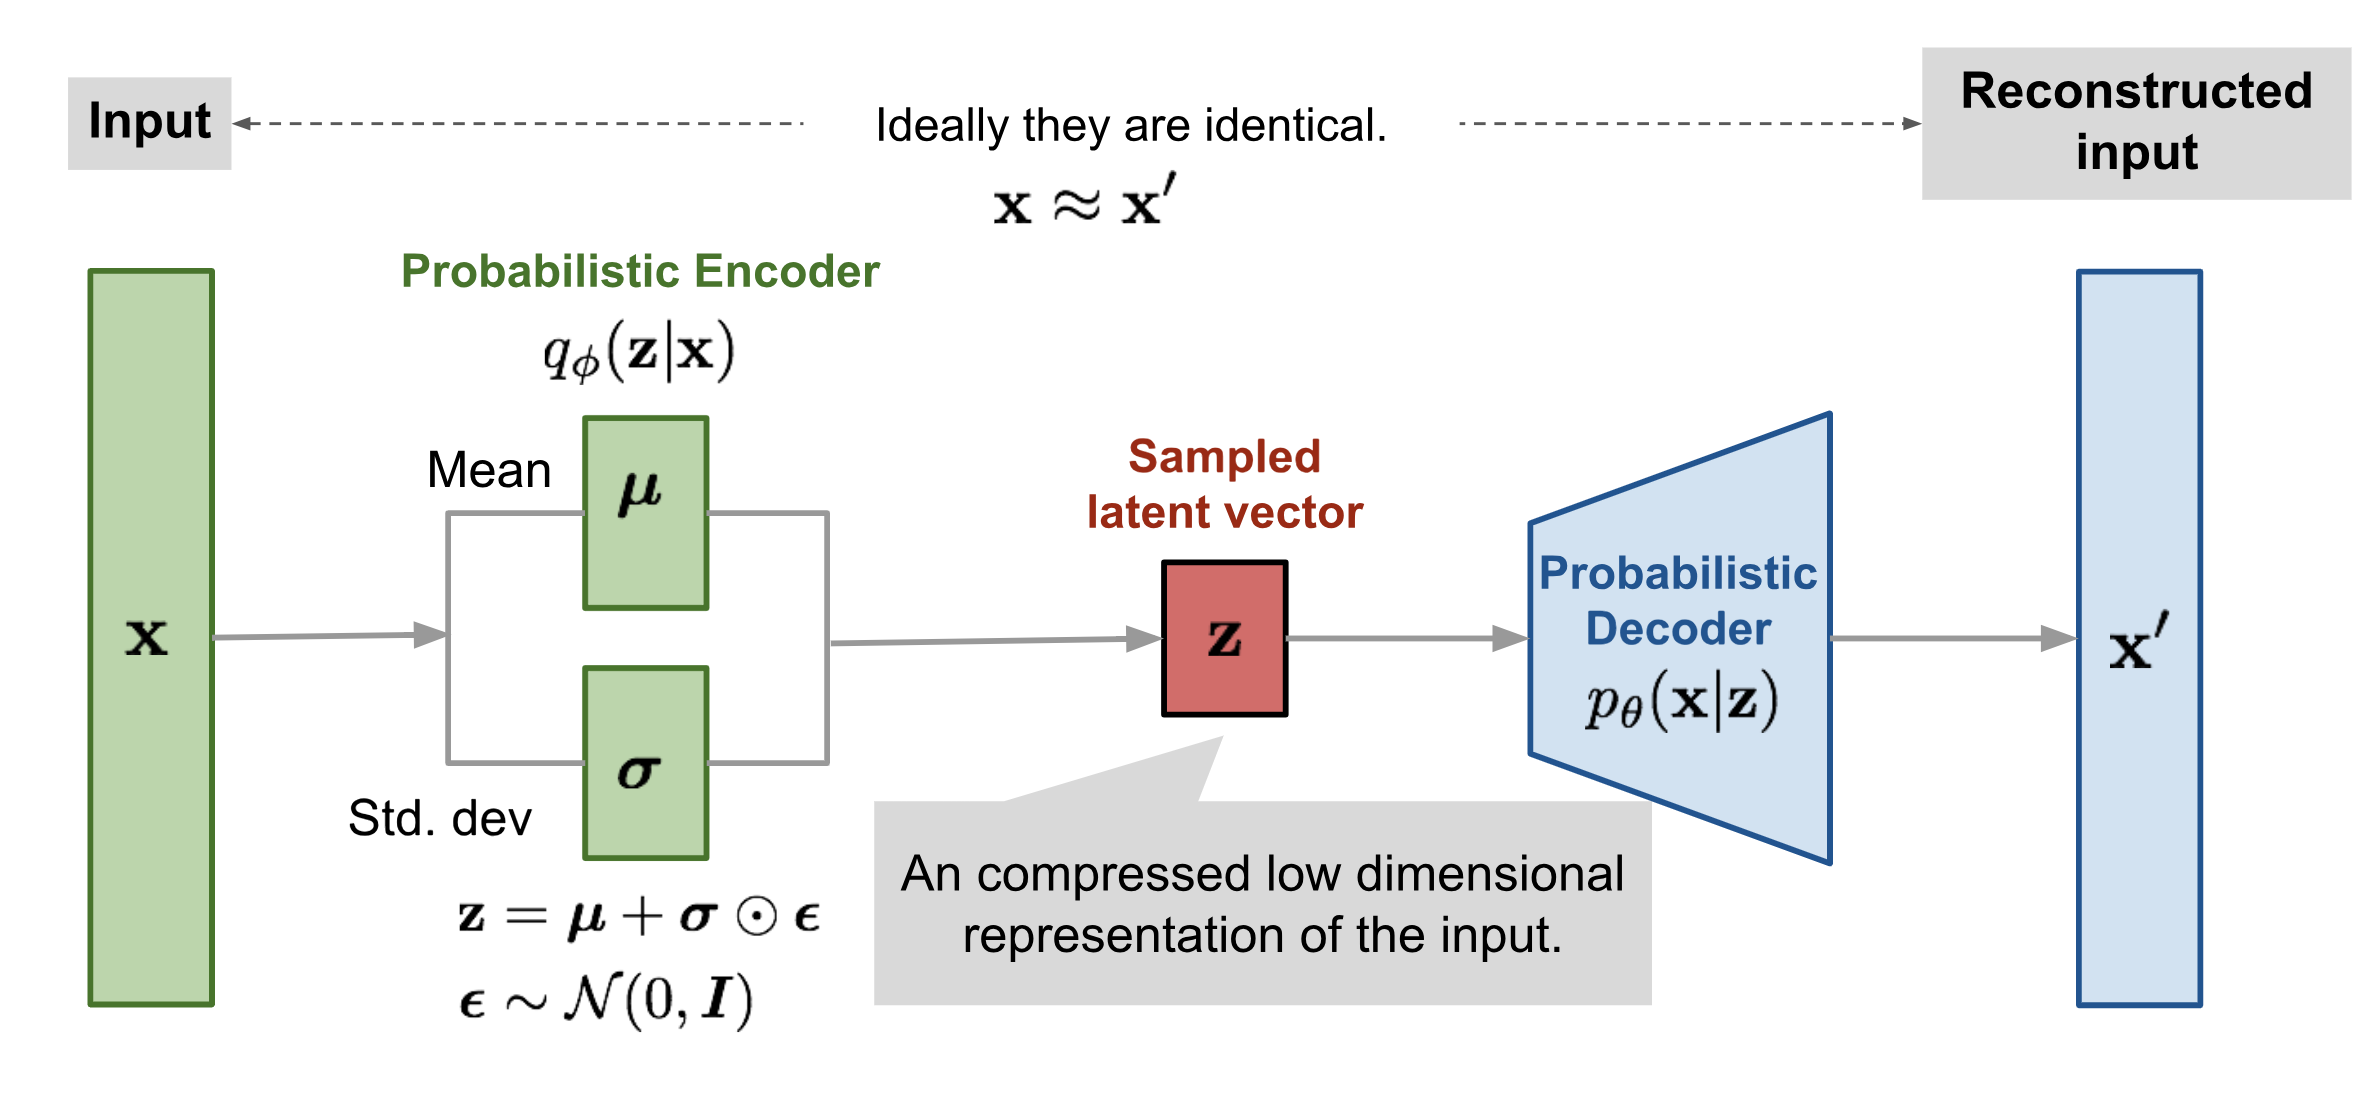
\includegraphics[width=\linewidth]{figs/vae-gaussian.png}
\end{figure}
 \hrule\medskip
{\scriptsize \href{https://lilianweng.github.io/lil-log/2018/08/12/from-autoencoder-to-beta-vae.html}{https://lilianweng.github.io/lil-log/2018/08/12/from-autoencoder-to-beta-vae.html}}
\end{frame}
%=======
\begin{frame}{Variational Autoencoder}
\begin{figure}[h]
	\centering
	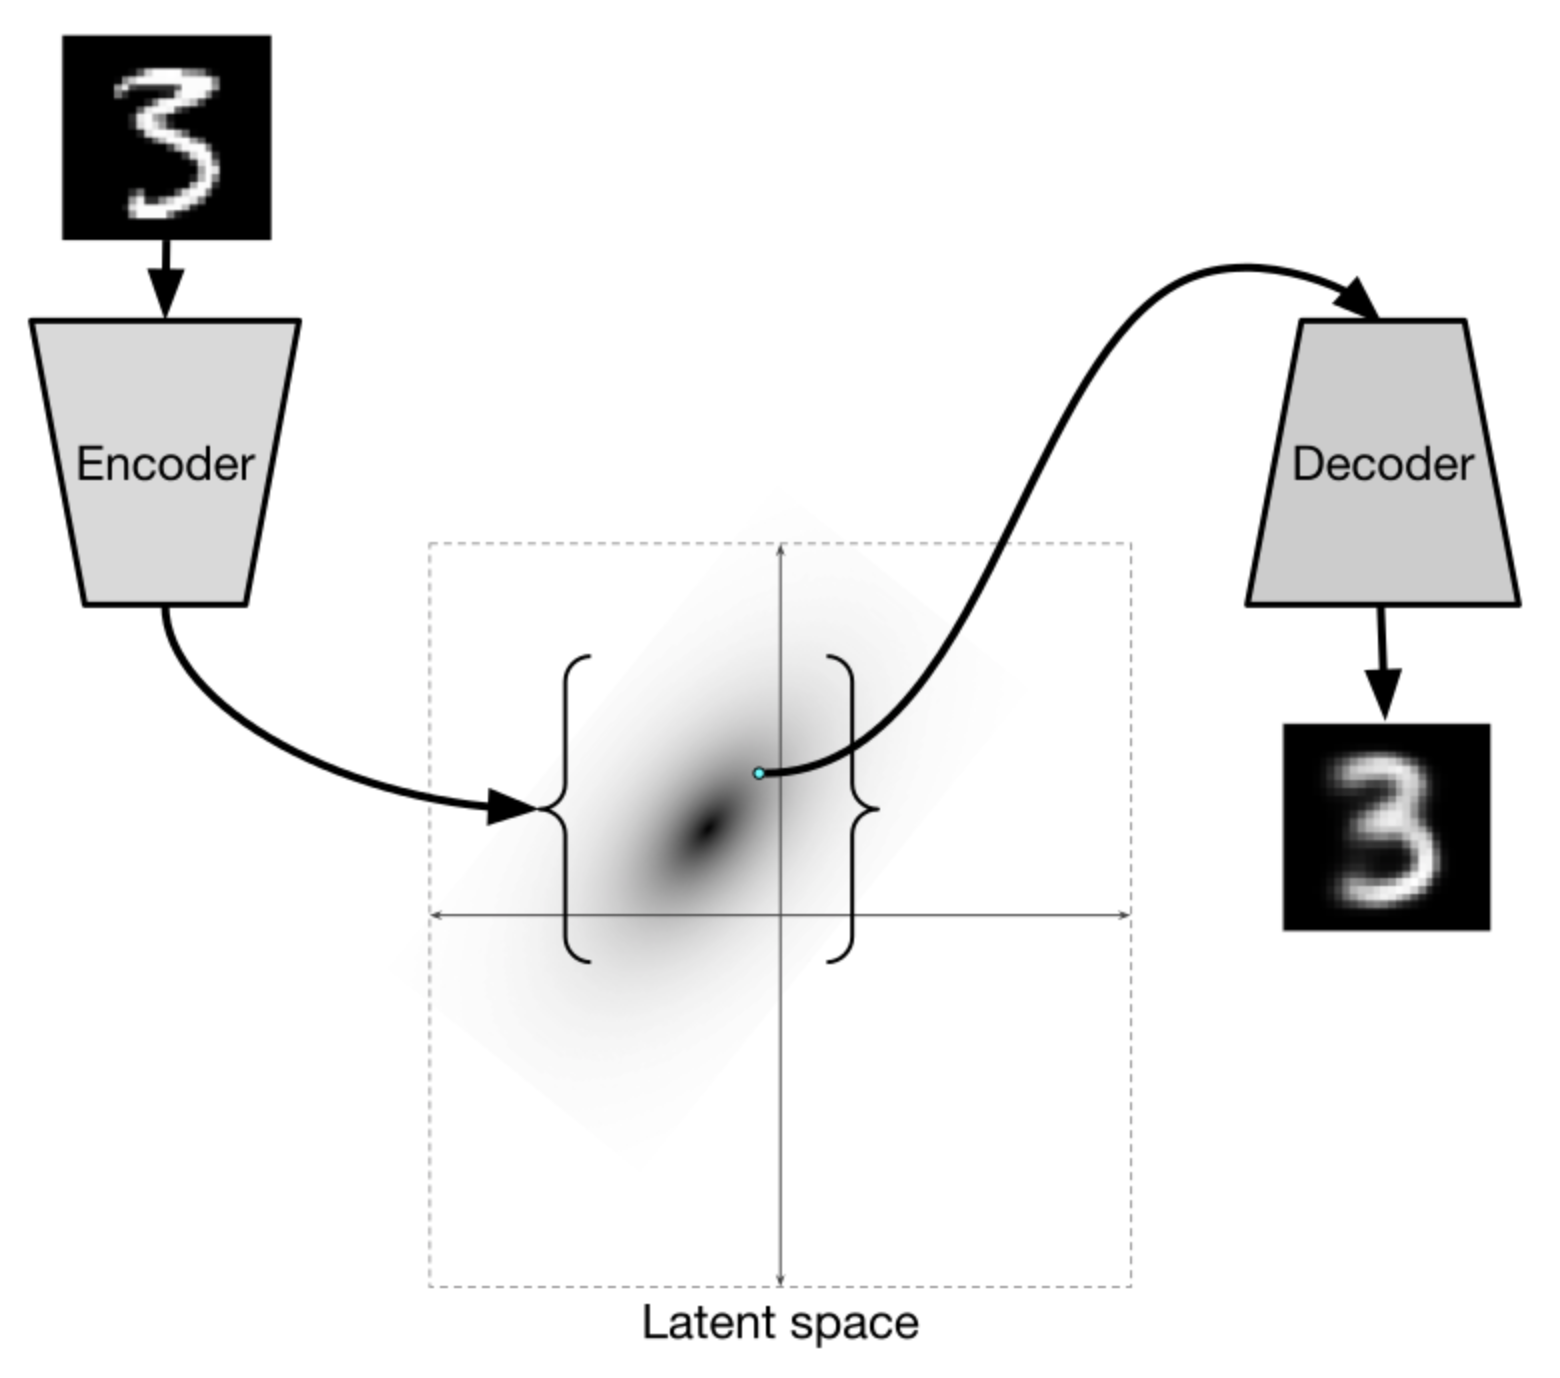
\includegraphics[width=.7\linewidth]{figs/VAE.png}
\end{figure}

\medskip\hrule\medskip
{\scriptsize Isaac Dykeman, \href{http://ijdykeman.github.io/ml/2016/12/21/cvae.html}{http://ijdykeman.github.io/ml/2016/12/21/cvae.html}}
\end{frame}
%=======
\begin{frame}{Variational Autoencoder}
Generation objects by sampling the latent space $\bz \sim \mathcal{N}(0, \mathbf{I})$
\begin{figure}[h]
	\centering
	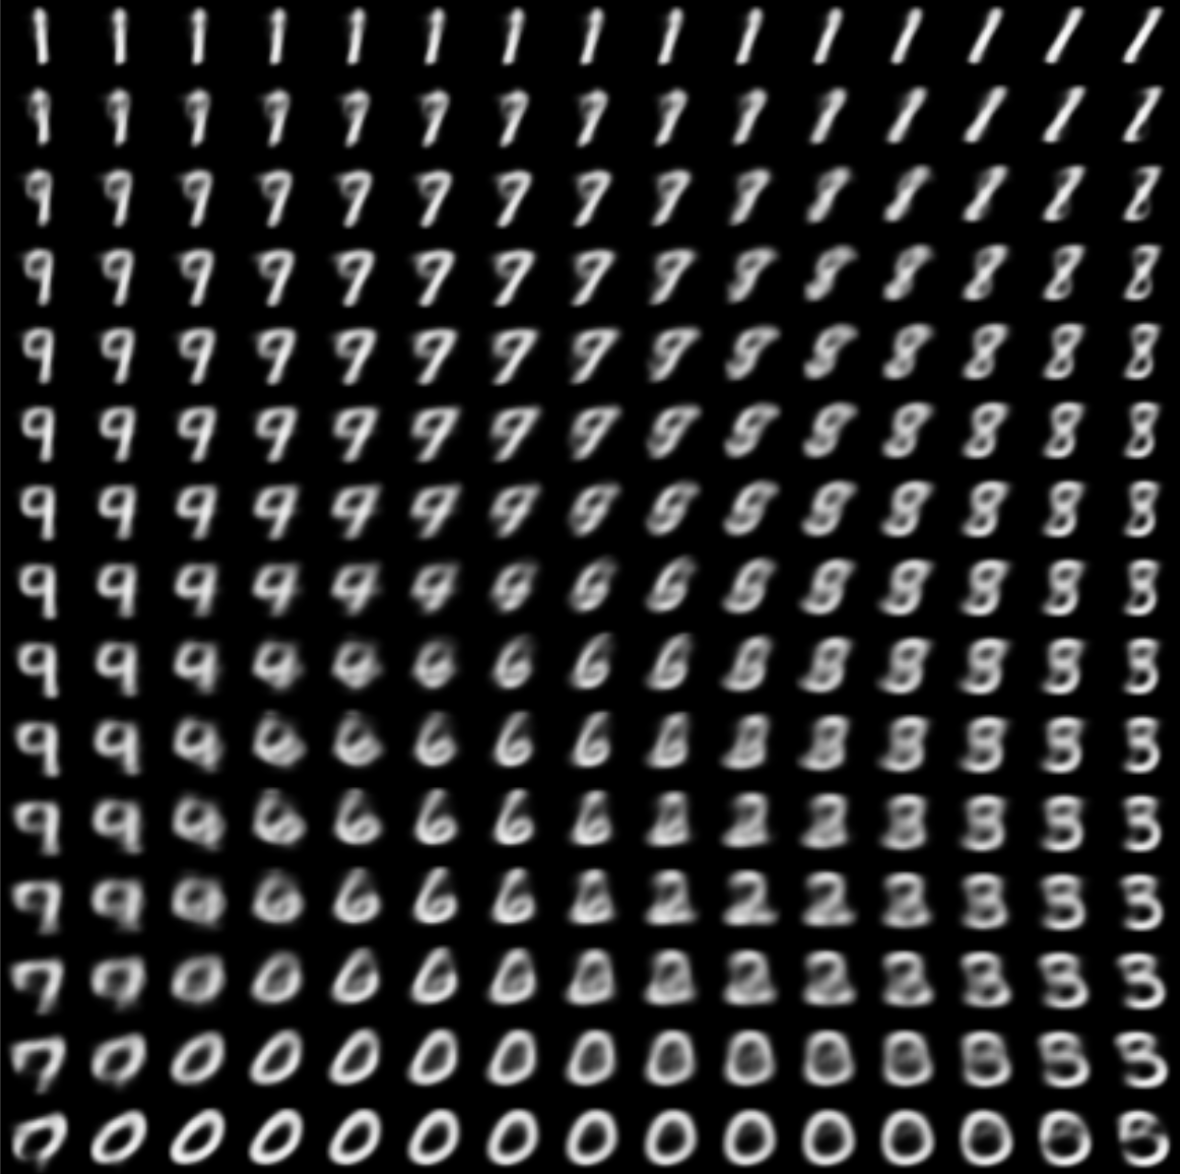
\includegraphics[width=.5\linewidth]{figs/vae_0.png}
\end{figure}
\vfill
\hrule\medskip
{\scriptsize \href{http://bit.ly/2w73aXB}{http://bit.ly/2w73aXB}}
\end{frame}
%=======
\begin{frame}{Bayesian framework}
    \begin{block}{Bayes theorem}
    \[
        p(\bt | \bx) = \frac{p(\bx | \bt) p(\bt)}{p(\bx)} = \frac{p(\bx | \bt) p(\bt)}{\int p(\bx | \bt) p(\bt) d \bt} 
    \]
    \begin{itemize}
        \item $\bx$ -- observed variables;
        \item $\bt$ -- unobserved variables (latent variables/parameters);
        \item $p(\bx | \bt)$ -- likelihood;
        \item $p(\bx)$ -- evidence;
        \item $p(\bt)$ -- prior;
        \item $p(\bt | \bx)$ -- posterior.
    \end{itemize}
    \end{block}
\end{frame}
%=======
\begin{frame}{Variational Lower Bound}
    We are given the set of objects $\bX = \{\bx_i\}_{i=1}^n$. 
    The goal is to perform bayesian inference on the latent variables $\bT = \{\bt_i\}_{i=1}^n$.
    \begin{block}{Empirical Lower BOund (ELBO)}
    \vspace{-0.3cm}
        \begin{multline*}
    		\log p(\bX) 
    		= \log \frac{p(\bX, \bT)}{p(\bT|\bX)} = \\ 
    		= \int q(\bT) \log \frac{p(\bX, \bT)}{p(\bT|\bX)}d\bT
    		= \int q(\bT) \log \frac{p(\bX, \bT) q(\bT)}{p(\bT|\bX) q(\bT)} d\bT = \\
    		= \int q(\bT) \log \frac{p(\bX, \bT)}{q(\bT)}d\bT + \int q(\bT) \log \frac{q(\bT)}{p(\bT|\bX)}d\bT = \\ 
    		= \mathcal{L} (q) + KL(q(\bT) || p(\bT|\bX)) \geq \mathcal{L} (q).
    	\end{multline*}
        \vspace{-0.3cm}
    \end{block}
\end{frame}
%=======
\begin{frame}{Mean field approximation}
    \begin{block}{Independence assumption}
    \vspace{-0.3cm}
    \[
    q(\bT) = \prod_{i=1}^k q_i(\bT_i), \quad \bT = [\bT_1, \dots, \bT_k], \quad \bT_j = \{ \bt_{ij}\}_{i=1}^n.
    \]
    \vspace{-0.3cm}
    \end{block}
    \begin{block}{Block coordinate optimization of ELBO for $q_j(\bT_j)$}
  
    {\footnotesize
    \vspace{-0.3cm}
        \begin{multline*}
    		\mathcal{L} (q)
    		= \int q(\bT) \log \frac{p(\bX, \bT)}{q(\bT)}d\bT
    		= \int \prod_{i=1}^k q_i(\bT_i) \log \frac{p(\bX, \bT)}{\prod_{i=1}^k q_i(\bT_i)}  \prod_{i=1}^k d \bT_i = \\
    		= \int \prod_{i=1}^k q_i \log p(\bX, \bT) \prod_{i=1}^k d \bT_i  
    		- \sum_{i=1}^k \int \prod_{j=1}^k q_j \log q_i \prod_{i=1}^k d \bT_i = \\
    		= \int q_j \left[\int  \log p(\bX, \bT) \prod_{i \neq j} q_i d \bT_i \right] d \bT_j - \\
    		- \int q_j \log q_j d\bT_j + \text{const}(q_j) \rightarrow \max_{q_j}
    	\end{multline*}
        \vspace{-0.3cm}}
    \end{block}
\end{frame}
%=======
\begin{frame}{Mean field approximation}
	\footnotesize
	\begin{block}{Block coordinate optimization of ELBO for $q_j(\bT_j)$}
		\vspace{-0.4cm}
	    \begin{multline*}
			\mathcal{L} (q) 
			= \int q_j \left[\int \log p(\bX, \bT) \prod_{i \neq j} q_i d \bT_i \right] d \bT_j
			- \int q_j \log q_j  d\bT_j + \text{const}(q_j) = \\
			= \int q_j \log \hat{p}(\bX, \bT_j) d \bT_j 
			- \int q_j \log q_j d\bT_j + \text{const}(q_j) \rightarrow \max_{q_j},
		\end{multline*}
		\[
		    \text{where } \log \hat{p}(\bX, \bT_j) = \mathbb{E}_{i \neq j} \log p(\bX, \bT) + \text{const}(q_j)
		\]
		\[
		    \mathbb{E}_{i \neq j} \log p(\bX, \bT) = \int \log p(\bX, \bT) \prod_{i \neq j} q_i d \bT_i.
		\]
		\vspace{-0.1cm}
		\begin{multline*}
    		\mathcal{L} (q)
    		= \int q_j (\bT_j) \log \hat{p}(\bX, \bT_j) d \bT_j - \int q_j(\bT_j) \log q_j(\bT_j) d\bT_j + \text{const}(q_j) = \\
    		 \int q_j (\bT_j) \log \frac{\hat{p}(\bX, \bT_j)}{q_j(\bT_j)} d\bT_j + \text{const}(q_j) = \\
    		= KL (q_j(\bT_j) || \hat{p}(\bX, \bT_j)) + \text{const}(q_j) \rightarrow \max_{q_j}.
    	\end{multline*}
    \end{block}
\end{frame}
%=======    
\begin{frame}{Mean field approximation}   
	 \begin{block}{Independence assumption}
		\vspace{-0.3cm}
		\[
		q(\bT) = \prod_{i=1}^k q_i(\bT_i), \quad \bT = [\bT_1, \dots, \bT_k], \quad \bT_j = \{ \bt_{ij}\}_{i=1}^n.
		\]
		\vspace{-0.3cm}
	\end{block}
	\begin{block}{ELBO}
		\vspace{-0.3cm}
	    \[
			\mathcal{L} (q) = KL (q_j(\bT_j) || \hat{p}(\bX, \bT_j))  + \text{const}(q_j) \rightarrow \max_{q_j}.
	    \]
	    \vspace{-0.3cm}
	\end{block}
	 \begin{block}{Solution}
	 	\vspace{-0.3cm}
		 \[
		    q_j(\bT_j) = \hat{p}(\bX, \bT_j)
		 \]
		 \[
		 	\log \hat{p}(\bX, \bT_j) = \mathbb{E}_{i \neq j} \log p(\bX, \bT) + \text{const}
		 \]
		 \[
		     \log q_j(\bT_j) = \mathbb{E}_{i \neq j} \log p(\bX, \bT) + \text{const}
		 \]
		 \vspace{-0.3cm}
	 \end{block}
\end{frame}
%=======
\begin{frame}{Mean field approximation}
	\begin{block}{ELBO}
		\[
			\mathcal{L} (q) = KL (q_j(\bT_j) || \hat{p}(\bX, \bT_j))  + \text{const}(q_j) \rightarrow \max_{q_j}.
		\]
		\vspace{-0.3cm}
	\end{block}
	\begin{block}{Solution}
		\vspace{-0.3cm}
		\[
			\log q_j(\bT_j) = \mathbb{E}_{i \neq j} \log p(\bX, \bT) + \text{const}
		\]
		\vspace{-0.3cm}
	\end{block}
	Let assume the following factorization: $\bT = [\bT_1, \bT_2] = [\bZ, \btheta]$, and restrict the class of probability distribution for $\btheta$ to Dirac delta functions:
	\[
		q_2 = q(\bT_2) = q(\btheta) = \delta(\btheta - \btheta_0).
	\]
	
	Under the restrictions the exact solution for $q_2$ is not reached.
\end{frame}
%=======
\begin{frame}{Mean field approximation}
	\begin{block}{General solution}
		\vspace{-0.3cm}
		\[
		\log q_j(\bT_j) = \mathbb{E}_{i \neq j} \log p(\bX, \bT) + \text{const}
		\]
		\vspace{-0.3cm}
	\end{block}
	\begin{block}{Solution for $q_1 = q(\bZ)$}
		\vspace{-0.3cm}
		\begin{multline*}
			\log q(\bZ) = \int q(\btheta) \log p(\bX, \bZ,  \btheta) d\btheta + \text{const} = \\
			= \int \delta(\btheta - \btheta_0) \log p(\bX, \bZ,  \btheta) d\btheta + \text{const} = \\
			= p (\bZ | \bX, \btheta_0) +  \text{const}.
		\end{multline*}
	\end{block}
	\vspace{-0.3cm}
	\begin{block}{EM-algorithm (E-step)}
		\vspace{-0.3cm}
	\[
		q(\bZ) = \argmax_q \mathcal{L} (q, \btheta^*) = \argmin_q KL(q || p) = p(\bZ| \bX, \btheta^*).
	\]
	\end{block}
\end{frame}
%=======
\begin{frame}{Mean field approximation}
	\begin{block}{ELBO}
		\[
			\mathcal{L} (q) = KL (q_j(\bT_j) || \hat{p}(\bX, \bT_j))  + \text{const}(q_j) \rightarrow \max_{q_j}.
		\]
	\vspace{-0.3cm}
	\end{block}
	\begin{block}{ELBO maximization w.r.t. $q_2 \equiv \theta_0$}
		\vspace{-0.3cm}
		\begin{align*}
			\mathcal{L} (q_2) &= KL (q(\btheta) || \hat{p}(\bX, \btheta))  + \text{const}(\btheta_0) \\ 
			&= \int q (\btheta) \log \frac{\hat{p}(\bX, \btheta)}{q(\btheta)} d\btheta + \text{const}(\btheta_0) \\
			& = \int q (\btheta) \log \hat{p}(\bX, \btheta) d\btheta  - \int q (\btheta) \log q(\btheta) d\btheta + \text{const}(\btheta_0) \\
			& = \int \delta(\btheta - \btheta_0) \log \hat{p}(\bX, \btheta) d\btheta  - \int \delta \log \delta d\btheta + \text{const}(\btheta_0) \\ 
			& = \int \delta(\btheta - \btheta_0) \log \hat{p}(\bX, \btheta) d\btheta + \text{const}(\btheta_0) 
		\end{align*}
		\vspace{-0.3cm}
	\end{block}
\end{frame}
%=======
\begin{frame}{Mean field approximation}
	
	\begin{block}{ELBO maximization w.r.t. $q_2 \equiv \theta_0$}
		\vspace{-0.3cm}
		\[
			\mathcal{L} (q_2) = \int \delta(\btheta - \btheta_0) \log \hat{p}(\bX, \btheta) d\btheta + \text{const}(\btheta_0) = \hat{p}(\bX, \btheta^0).
		\]
	\end{block}
	\vspace{-0.3cm}
	\[
		\log \hat{p}(\bX, \bT_j) = \mathbb{E}_{i \neq j} \log p(\bX, \bT) + \text{const}
	\]
	\begin{align*}
		\log \hat{p}(\bX, \btheta) &= \mathbb{E}_{q_1} \log p(\bX, \bZ, \btheta) + \text{const} \\
		&= \int q(\bZ) \log p(\bX, \bZ|  \btheta) d\bZ + \log p(\btheta)+ \text{const}
	\end{align*}
	\vspace{-0.3cm}
	\begin{block}{EM-algorithm (M-step)}
		 \[
		 	\mathcal{L}(q, \btheta) =	\int q(\bZ) \log \frac{p(\bX, \bZ | \btheta)}{q(\bZ)}d\bZ \rightarrow \max_{\btheta}
		 \]
	\end{block}
\end{frame}
%=======
\begin{frame}{Mean field approximation}
    \begin{block}{Solution}
    \[
        \log q_j(\bT_j) = \mathbb{E}_{i \neq j} \log p(\bX, \bT) + \text{const}
    \]
    \end{block}

	\begin{block}{EM algorithm}
	\begin{itemize}
		\item Initialize $\btheta^*$;
		\item E-step
		\[
			q(\bZ) = \argmax_q \mathcal{L} (q, \btheta^*) = \argmin_q KL(q || p) =
			 p(\bZ| \bX, \btheta^*);
		\]
		\item M-step
		\[
			\btheta^* = \argmax_{\btheta} \mathcal{L} (q, \btheta);
		\]
		\item Repeat E-step and M-step until convergence.
	\end{itemize}
	\end{block}
\end{frame}
%=======
\begin{frame}{Summary}

\begin{itemize}
	\item Latent variable models introduce latent variables to the initial probabilistic model to make distribution $p(\bx | \btheta)$ tractable.
	\item To solve the MLE problem LVM optimizes variational lower bound.
	\item EM-algorithm is an iterative algorithm which allows to optimize the variational lower bound.
	\item VAE model is a LVM, encoder is a variational distribution, decoder is a likelihood model.
	\item Mean field approximation is a general form of variational inference (EM-algorithm is just a special case).
\end{itemize}
\end{frame}
%=======
%--------------------------------------------------------------------------------
\section{Conclusion}
%--------------------------------------------------------------------------------

\end{document} 